% -*- coding: utf-8 -*-
\newpage
\section{Optimisation of the code}

The Amsterdam Modeling Suite is a large and evolving code composed of
multiple modules, each with its own features and interfaces. Over time it
has transitioned from early \fortran dialects to modern standards and has
developed a \python library to coordinate the \ams
engines. Despite extensive documentation and developer tooling, two
avenues for improvement remain central to long-term sustainability:
$i$) refactoring for clarity and maintainability, and $ii$) targeted
optimisations for memory footprint and runtime.

\subsection{Memory Optimisation}

In previous versions, properties evaluated at \glspl{CP} were stored in a
single preallocated two-dimensional array. Its first dimension assumed an upper
bound of $256$ \glspl{CP} per atom (multiplied by the number of atoms), while
the second dimension listed the properties per \gls{CP} ($27$ entries, one
unused). This conservative approach wasted memory for realistic systems, where
the actual number of \glspl{CP} is markedly lower than the imposed maximum.

\subsubsection{Estimating a Upper Bound}

To reduce memory usage without compromising functionality, we analysed the
theoretical upper limits for the number of bonds, rings, and cages in a system
as a function of the number of atoms. Because the identification of \glspl{NNA}
occurs after memory allocation, a buffer must be included to account for their
possible presence. We adopt a conservative limit of either ten additional
attractors or 10\% of the number of atoms, whichever is larger.

Then to estimate the number of bonds, we consider a hypothetical ---albeit
physically unrealistic--- scenario in which every atom is bonded to every other
atom: $\max(\text{BCP}) = (n - 1)\sfrac{n}{2}$, \noindent where $n$ is the
number of atractors.  To estimate the maximum number of rings, we consider the
upper limit based on polygonal connectivity, assuming no subsets:
$\max(\text{RCP}) = (n - 3)\sfrac{n}{2} + 1$.  For cages, if we consider only
convex polyhedra composed of triangular faces, we derive to $\max(\text{CCP}) =
6n - 24$.

While such estimates exceed what occurs in chemically realistic
systems, they provide conservative bounds for safe memory allocation.
%
\begin{align}
  \max(\text{CP}) = n^2 + 4n -23
\end{align}

\subsubsection{Dynamic Allocation Strategy}

The original implementation allocated more memory than the theoretical upper
limit discussed above. While this ensured correctness, it left room for
improvement. Our aim was therefore to design a strategy that remains close to
the theoretical bound for small systems, but grows more moderately with system
size in order to reduce unnecessary overhead for large systems.  

\vspace{0.5cm}%

In constructing such a function, we also examined definitions based on
piecewise regimes, where different growth laws are applied in distinct regions
of system size. While these approaches can be tuned to follow the theoretical
limit more closely in certain ranges, they inevitably introduce \texttt{if}
statements into the code, which reduces readability.  Since our goal was not to
optimise memory allocation with mathematical precision, but rather to provide a
practical and transparent strategy, we chose to avoid such constructions. 

\vspace{0.5cm}%

Several candidates were considered, as illustrated in
Figure~\ref{memory_strategies}. Ultimately, we selected the simplest
formulation, prioritising clarity.  Although this choice slightly overallocates
memory for small systems, the overhead is negligible in practice. More
importantly, the gradual growth at larger system sizes ensures that the code
remains both efficient and scalable.

\newpage
\vspace*{1.0cm}%
\begin{lstlisting}[language=Fortran, style=mystyle]
   integer, parameter :: numCPprops = 26 ! Number of properties per critical point

   ! Adjusted number of atoms for periodic systems and non-periodic systems                                                         
   nVectors = 0_KINT 
   if (present(numLatticeVectors)) nVectors = numLatticeVectors                                                                     
   maxCP = numAtoms + 3**nVectors                                                                                                   
                                                                                                                                           
   ! Maximum number of critical points                                                                                              
   maxCP = max(maxCP + 10, maxCP + maxCP/10) ! 10 NNAs or 10 % NNAs                                                     
   maxCP = int(50*sqrt(real(maxCP))*(1 - exp(-real(maxCP)/50)))                                                                        
   allocate(self%cpmat(maxCP, numCPprops), stat=ialloc) 

   ! Check the allocation status; and error is fatal if first argument is 0
   call chckmem(0, moduleName//'::cpmat', ialloc)
\end{lstlisting}

% \newpage
\begin{figure}[h]
  \centering
  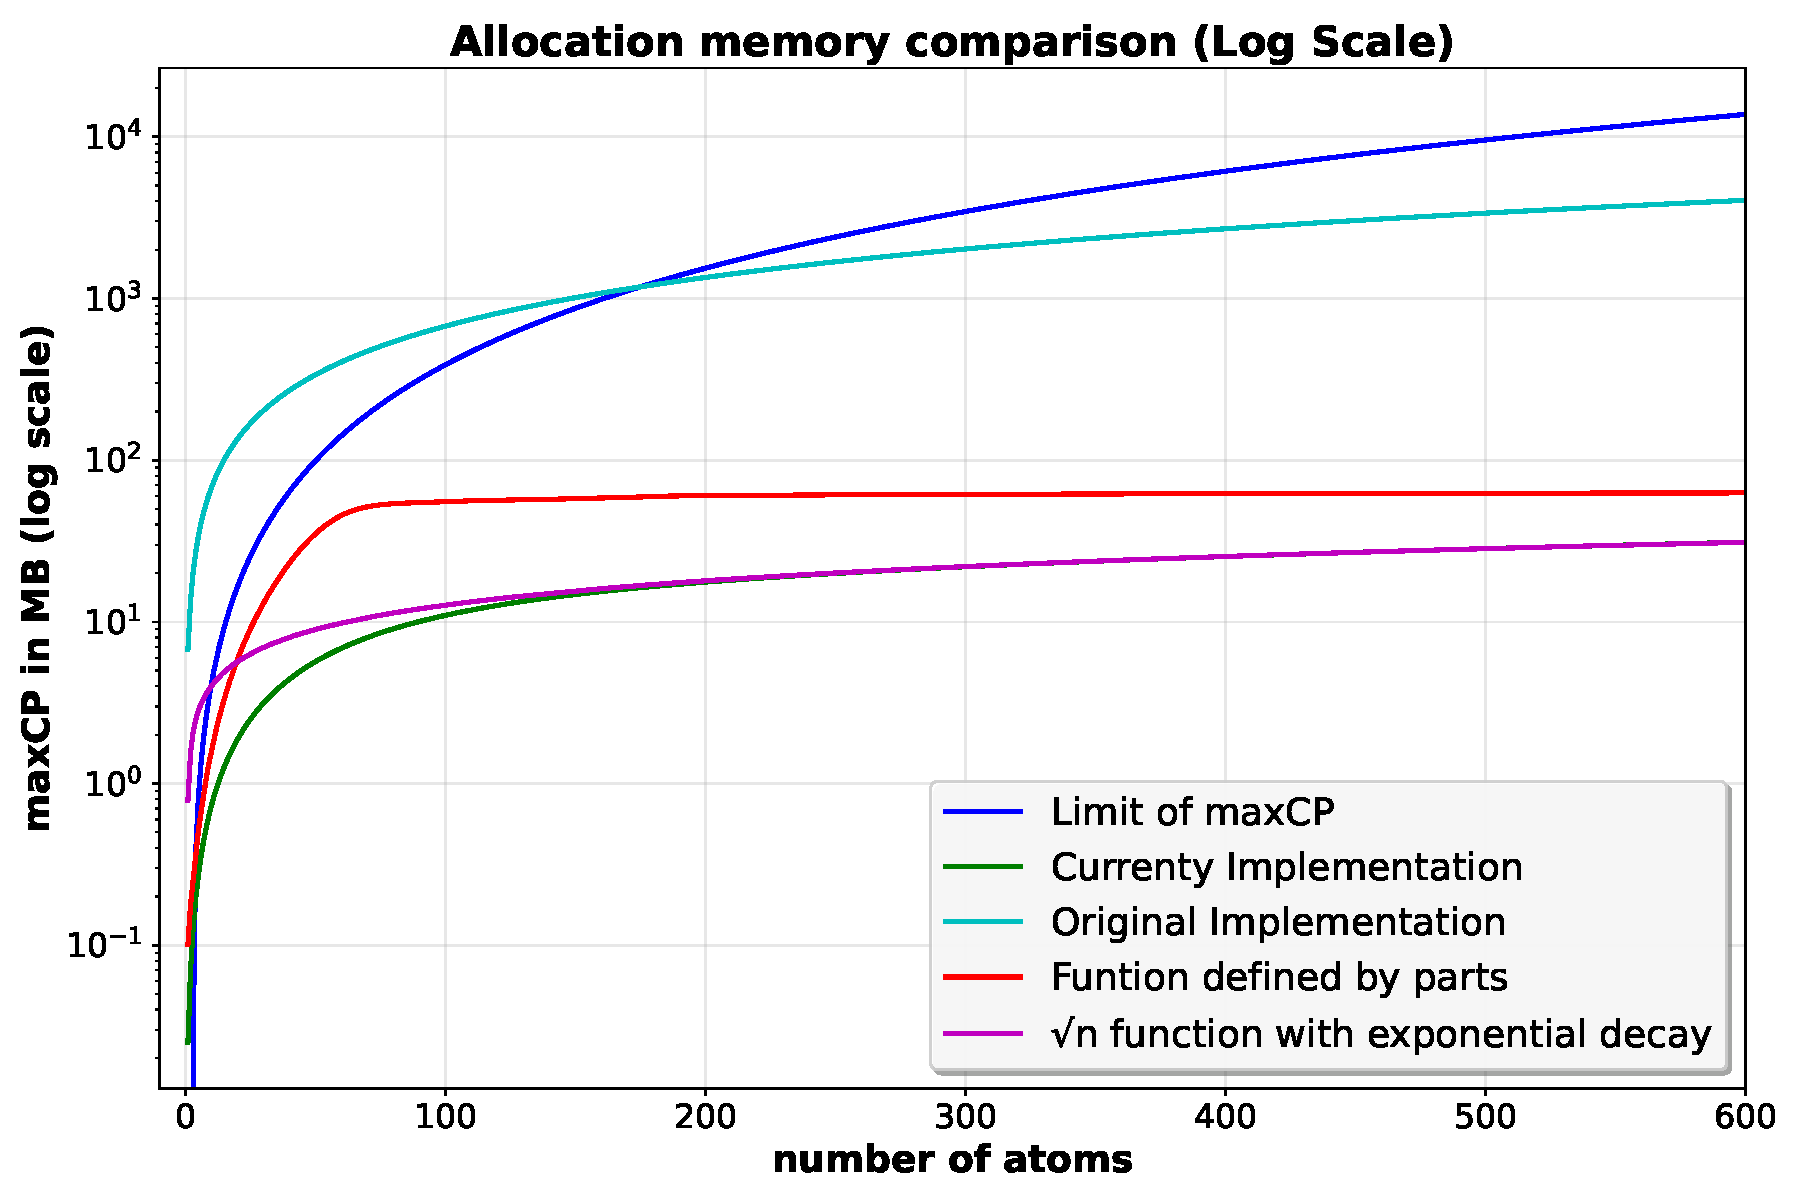
\includegraphics[width=0.7\textwidth]{img/memory_optimisation_curve.pdf}
  \caption{Comparison of alternative memory allocation strategies as
           function of system size.}
  \label{memory_strategies}
\end{figure}

\newpage
\subsection{Refactoring}

Several parts of the code were originally written in a style that new
developers might find difficult to follow and, more importantly, to maintain.
For instance, the \subroutine \texttt{UpdateAIMTerms} called two separate
\subroutines which computed almost identical quantities, differing only in the
treatment of a few variables, as shown in the code excerpt below.

\begin{lstlisting}[language=Fortran, style=mystyle]
   if (baderEnergy) then 
      call elf(lblock,fragment%nspin,rho0,rho1,tau,elfu) 
      call CalcAtomPropEnergy(gridAtomMap, xyzatm, & 
                              coords,wghts,rho0,rho1,rho2,ntr,op,  &  
                              tau,vXC,EpsXC,vNuc,vHartree,elfu, & ! Extra variables
                              fden,aimProperty,orbgrd,atomNbPts,inpatm) 
   else 
      call CalcAtomProp(gridAtomMap, xyzatm, & 
                        coords,wghts,rho0,rho1,rho2,ntr,op,  & 
                        fden,aimProperty,orbgrd,atomNbPts,inpatm)
   end if
\end{lstlisting}

% \newpage
Merging these two \subroutines (\texttt{CalcAtomPropEnergy} and
\texttt{CalcAtomProp}) eliminated duplicated logic, improved readability, and
simplified the overall flow of the program.

\begin{lstlisting}[language=Fortran, style=mystyle]
   if (baderEnergy) call elf(lblock, fragment%nspin, rho0, rho1, tau, elfu)
   call CalcAtomProperties(gridAtomMap, xyzatm, coords, wghts, &
                           rho0, rho1, rho2, op, &
                           tau, vXC, EpsXC, vNuc, vHartree, elfu, & ! Ignore if not needed
                           fden, aimProperty, orbgrd, atomNbPts, inpatm) 
\end{lstlisting}

The refactored \subroutine has an extra \texttt{if} statement to use the extra
variables, the \subroutine is the one we describe in
Algorithm~\ref{updateaimterms}.

% \begin{lstlisting}[language=Fortran, style=mystyle]
%    ! ... 
%    do i = 1, nblocksize
%       ! ... 
%       aimProperty(atom, 1) = aimProperty(atom, 1) + f*weight ! density
%       ! ... 
%       if (baderEnergy) then
%          aimProperty(atom,11) = ! ... Bader ELF
%          aimProperty(atom,12) = ! ... Bader Ts
%       end if
%       ! ...
% \end{lstlisting}

\newpage
Other refactoring steps focused on improving efficiency. The inclusion of
precomputing factors outside of loops rather than repeatedly recalculating them
was a common pattern throughout the codebase.  We display an example in the
code snippets below:

\begin{lstlisting}[language=Fortran]
  ! Old code
  ! Loop over the number of Critical Points
  ! the name nna is not clear; can be understood as number of non-nuclear attractors]
  DO i = 1, nna 
    ! Factors over computed; every loop of i the same factors are computed
    DO ii=1,36
       newAbscissae(ii,1) = pi*abscissae(ii)+pi
       newAbscissae(ii,2) = pi/two*abscissae(ii)+pi/two
    END DO
    ! The scalars can be computed outside the integral
    integral = 0.0_KREAL 
    DO ii=1,36
       DO jj=1,36
          integrand = SQRT(! Code omitted for brevity...
          integral  = integral + pi*pi/two*weights(ii)*weights(jj)*integrand 
       END DO
    END DO 
    ! ...
\end{lstlisting}

% \newpage
\begin{lstlisting}[language=Fortran]
  ! New code
  ! Pre-compute the factors outside the integral loop
  do i = 1, 36
     newAbscissae(i,1) =     pi*abscissae(i) + pi
     newAbscissae(i,2) = halfpi*abscissae(i) + halfpi
  end do
  do i = 1, ncp ! Loop over the number of Critical Points
     integral = 0.0_KREAL
     do itheta = 1, 36
        do iphi = 1, 36
           integrand = SQRT(! Code omitted for brevity...
           integral  = integral + weights(itheta)*weights(iphi)*integrand
        end do
     end do
     integral = pi*halfpi*integral ! Scale the integral outside the loop
     ! ...
\end{lstlisting}

\newpage
Encapsulation was another key aspect: new \modules were created to group
related functionality. For example, a dedicated \module was introduced for
handling plain-text output and binary file writing (see
Appendix~\ref{rkf_files}), and another \module for general mathematical
utilities. Likewise, functionality for following the gradient path was placed
in a separate \module, ensuring that a single, consistent \subroutine could be
applied to bonds, rings, and cages.

\vspace*{1em}%
Previously, the Runge-Kutta method was implemented directly inside the bond
path \subroutine and the \subroutine dedicated to assigning grid
points to basins, making it inaccessible to other parts of the code and leading
to duplicated code. By encapsulating the method in a standalone \subroutine, it
became reusable across the \gls{QTAIM} partition, enabling algorithms such as
Algorithm~\ref{brc_cpAlgo} to be written without redundant implementations. In
the same spirit, all Graph Theory and Geometry features were conceived from the
outset as independent \modules (Subsection~\ref{graph_theory} and
Appendix~\ref{icosphereGeo}).

\vspace*{1em}%
Finally, additional comments and explicit parameter definitions were introduced
to improve readability and maintainability. In the main \module where all
\gls{QTAIM} variables are declared, comments now provide a clear map of array
indices to the corresponding physical properties (\eg\ density, dipole and
quadrupole moments, Laplacian, spin density, basin volume).
Similarly, in the \module responsible for computing properties at \glspl{CP},
integer parameters were defined to label array indices such as
coordinates, density, gradient, Hessian, signature, and eigenvectors. These
additions reduce ambiguity, make the code self-documenting, and simplify future
modifications by replacing hard-coded indices with descriptive constants.

